%!TEX root = ../main.tex
\chapter{光阴极微波电子枪中的超低束流发射度的基本理论}
\label{chap:theory}

要探究光阴极微波电子枪中的极限束流发射度,首先要对光阴极电子枪中的物理有一个全面的认识,本章就来介绍光阴极电子枪中的基本物理概念与公式。

\section{束流相空间与束流发射度}
\subsection{束流相空间}
束流是由若干粒子组成的,每个粒子的运动状态都可以用一个六维向量来描述,即粒子的空间坐标 $(x, y, z)$ 和动量空间坐标 $(p_x, p_y, p_z)$ 的组合。那么在六维坐标系(相空间)中 $(x, y, z, p_x, p_y, p_z)$,每个粒子都可以用其中一个点代表。将束流中每个粒子都画在该坐标系中,就是束流的相空间分布。图 \ref{fig:phase-space}(来自维基)给出了一个束团的相空间分布在二维坐标系 $(x, p_x)$ 中的投影分布,这样一个投影分布称为束流的二维相空间分布。
\begin{figure}[htbp]
\centering
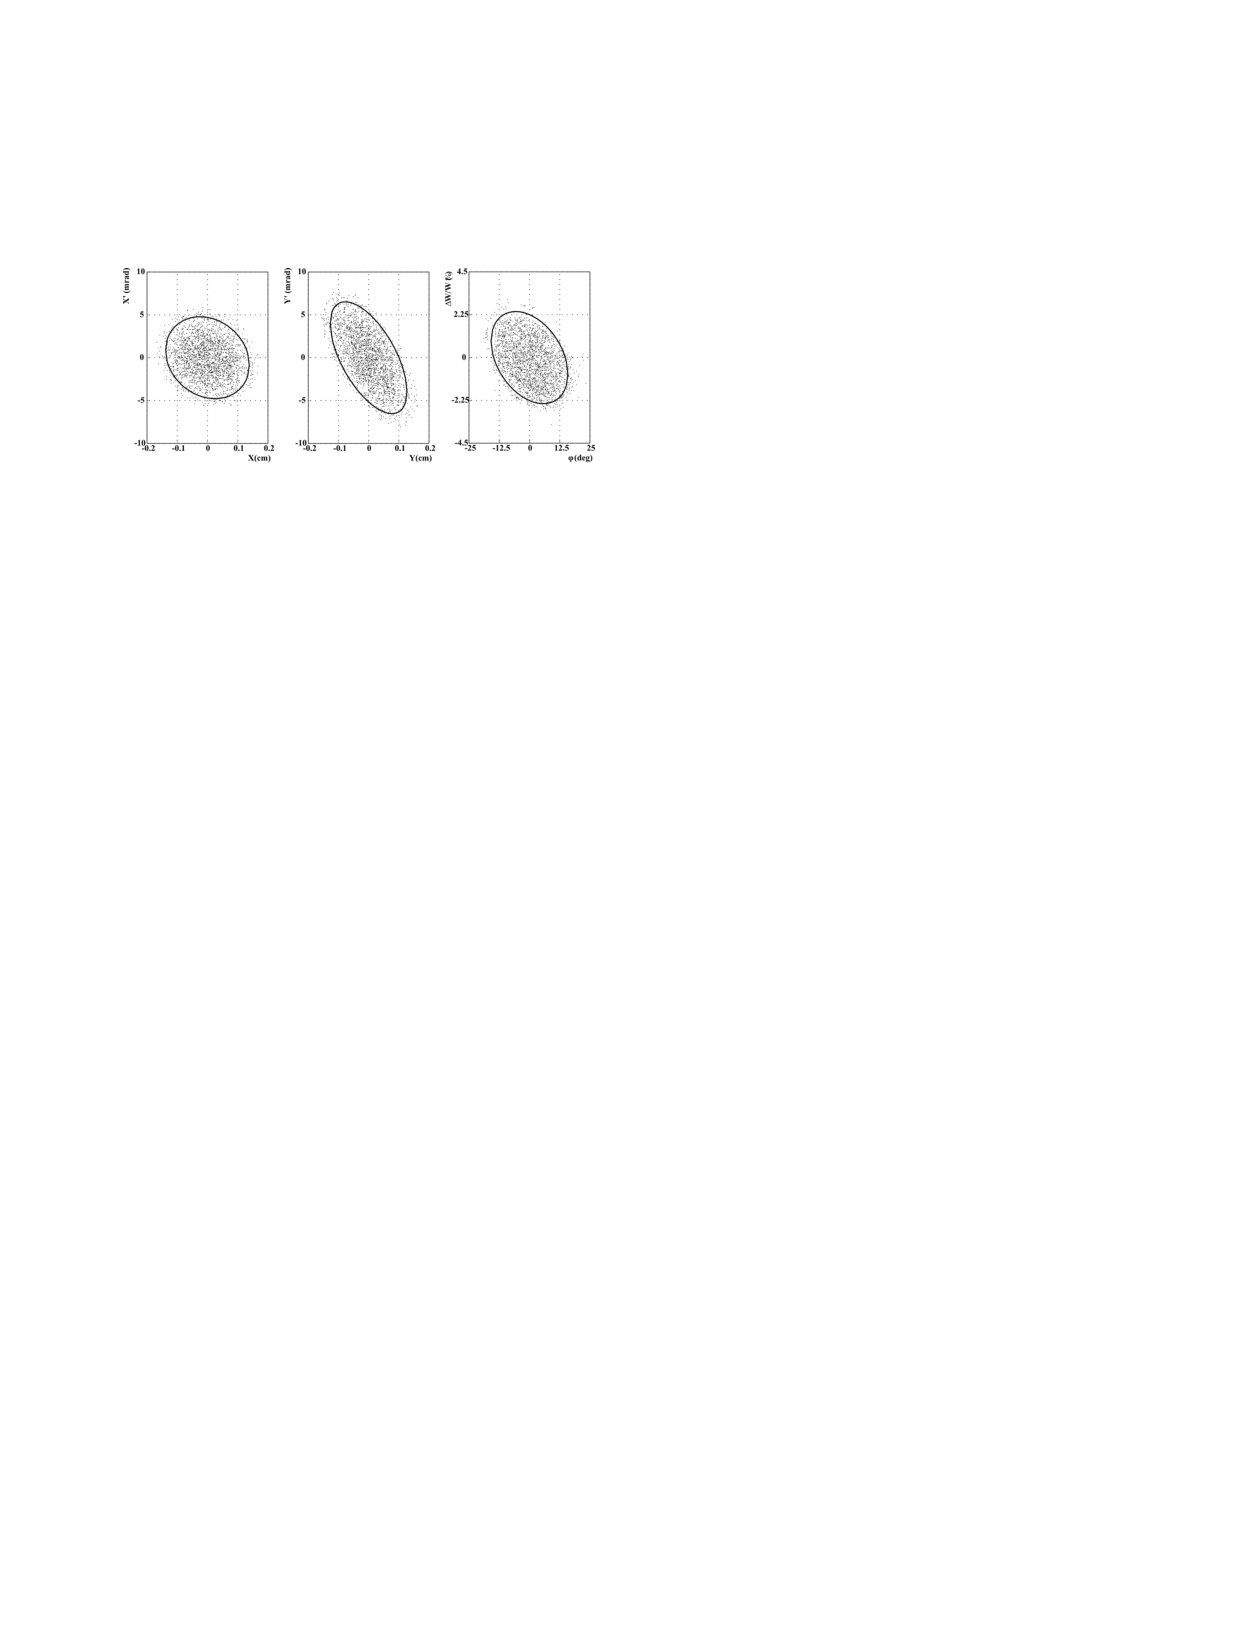
\includegraphics[width=0.6\textwidth]{phasespace}
\caption{\label{fig:phase-space} 一个束团在 $x$ 方向的二维投影相空间分布}
\end{figure}

\subsection{束流发射度}
刘维尔定理指出,若粒子间无相互作用力,且束流所受外力均为保守力,则相空间的体积不变,这个不变的体积就称为束流的发射度。若束流的三方向无耦合(即三方向 $x, y, z$ 的运动互相无影响),则刘维尔定理也对三方向的二维相空间成立,此时三方向上的二维相空间的面积就称为相应方向的发射度。对于 x 方向的相空间分布,有下面的统计发射度定义:
\begin{equation}
\varepsilon = \sqrt{\langle x^2\rangle\langle p_x^2\rangle-\langle xp_x\rangle^2}
\label{eq:stat-emit-1}
\end{equation}
其物理意义是用椭圆去拟合相空间分布,求出的椭圆面积除以 $\pi$ 就是该相空间分布的发射度。

在加速器物理中,由于束流中粒子之间存在空间电荷力,刘维尔定理不能精确成立;然而加速器中的束团普遍具有较好的柱对称性,以及束团中粒子数极为巨大,可近似将束流看做连续体,所以粒子的空间电荷效应往往可以等效成一个保守外力,在这种情况下,束流的发射度依然近似为常数。

\section{光阴极微波电子枪中存在的束流发射机制}

\subsection{光电发射}
光电效应是指光束照射在金属表面会使其发射电子的物理现象,发射出的电子被称为光电子。对于特定金属而言,入射光频率必须大于某特定值才能产生光电效应,光电效应的发生与否与入射光强度没有关系。光电效应是一种量子效应,无法用 Maxwell 体系的经典电磁理论解释,必须借助光量子的概念才能解释。

光电效应可用下面著名的公式描述:
\[
E = h\nu-\phi
\]
其中$E$是出射光电子最大能量,$h\nu$为入射光子能量,$\phi$称为金属的逸出功或功函数(work function)。

\subsubsection{单光子光电效应与多光子光电效应}
人们在刚刚认识光电效应本质时,认为只有光子能量高于金属逸出功的时候才能产生光电发射。随着激光技术的发展,高功率激光被应用于研究中,此时发现了高阶光电效应:光子能量低于金属逸出功时,只要激光功率足够强,也能产生光电发射,这就是多光子光电效应现象。

\paragraph{单光子光电效应}
单光子光电效应就是金属内电子吸收单个光子的光电效应。

金属内处于费米能级(Fermi Energy)以下的束缚态电子吸收单个光子跃迁到高能态,进而成为自由电子向四周运动;经过若干次散射(能量损失)后部分高能态电子会到达金属表面,其中又有部分电子具有足够能量,克服金属表面势垒后从金属表面逸出,成为光电子。

1931 年 R. Fowler 研究了光电发射中光电流随入射光子能量变化曲线的拖尾现象。他采用简并电子气的观点,并假设:
	\begin{itemize}
	\item 吸收光子后电子的能量略高于克服表面势垒所需能量,因此忽略电子间散射作用
	\item 所有沿阴极法向的动能与吸收的光子能量之和大于克服阴极表面势垒所需能量的电子都可从表面逃逸,这种电子叫做可出射电子
	\item 光电流正比于可出射电子数
	\end{itemize}
	根据以上假设,R. Fowler 获得了光电发射电流 $I$ 的表达式,成功地揭示了拖尾现象的机理。1933 年 L. Dubridge 扩充了 Fowler 的理论,计算了光电发射中光电子的能谱,因此该理论被称为 Fowler-Dubridge 理论。

Fowler-Dubridge 理论中光电流可以简单推导如下:假定阴极表面法向沿 $+x$ 方向,利用简并电子气的速度分布公式,可以得到电子密度随 $v_x$ 的分布如下:
	\[
	n(v_x) = \frac{4\pi kT}{m}\left(\frac{m}{h}\right)^2\log\{1+e^{(\mu-\frac{1}{2}mv_x^2)/kT}\}
	\]
	根据 Fowler 的第二条假设,单位体积内所有可出射的电子数为:
	\begin{eqnarray*}
	&N &= \int_{\frac{1}{2}mv_x^2=\phi_w+\mu-h\nu}^{\infty}n(v_x)dv_x\\
	&&= \frac{2\pi kT}{m}\left(\frac{2kT}{m}\right)^{1/2}\left(\frac{m}{h}\right)^3\int_0^{\infty}\frac{\log\{1+e^{-y+(h\nu-\phi_w)/kT}\}}{\{y+(\mu+\phi_w-h\nu)/kT\}^{1/2}}dy
	\end{eqnarray*}
	根据 Fowler 的第一条假设,上式积分分母中的 $y$ 相比于第二项可以忽略,所以上式可简化为:
	\[
	N = \frac{2\sqrt{2}\pi m^{3/2}}{h^3}\frac{(kT)^2}{(\mu+\phi_w-h\nu)^{1/2}}\int_0^{\infty}\log\{1+e^{-y+(h\nu-\phi_w)/kT}\}dy
	\]
	令 $F(x) = \int_0^{\infty}\log(1+e^{-y+x})dy$,则:
	\[
	N = \frac{2\sqrt{2}\pi m^{3/2}}{h^3}\frac{(kT)^2}{(\mu+\phi_w-h\nu)^{1/2}}F\left(\frac{h\nu-\phi_w}{kT}\right)
	\]
	根据 Fowler 的第三条假设,光电流 $I$ 正比于可出射电子数 $N$,我们就得到单光子发射光电流:
	\begin{equation}
	I = CT^2F\left(\frac{h\nu-\phi_w}{kT}\right)
	\end{equation}
	其中 $C$ 为常数,$T$ 为电子气温度,$F(x)$ 为 Fowler 函数,可以展成下面级数:
	\[
	F(x) =
	\begin{cases}
	e^x-\dfrac{e^{2x}}{2^2}+\dfrac{e^{3x}}{3^2}-\cdots & x \le 0\\[10pt]
	\dfrac{\pi^2}{6}+\dfrac{x^2}{2}-\left[e^{-x}-\dfrac{e^{-2x}}{2^2}+\dfrac{e^{-3x}}{3^2}-\cdots\right] & x > 0
	\end{cases}
	\]
	Fowler 函数的特征是在 $x < 0$ 时,其值随 $x$ 的减小而迅速衰减。这个特性意味着波段合适的激光可以作为阴极的发射开关,即光电发射具有良好的可控性。

单光子光电发射中,光电子数目(光电子产额)与入射光强度成正比,因此又被称为线性光电效应,可以定义光阴极的量子效率 QE 如下:
	  \begin{equation}
	  QE = \frac{N_e}{N_p} = \frac{Q/e}{IS\tau/h\nu} = \frac{J}{I}\cdot\frac{h\nu}{e}
	  \end{equation}
	  其中$N_e$为出射光电子数,$N_p$为入射光子数,$Q$是出射束团电荷量,$J$是出射电流密度,$I$是入射光功率密度,$h\nu$为入射光子能量,$e$为电子电荷量,$S$为入射光横向面积,$\tau$为入射光脉宽

\paragraph{多光子光电效应}
多光子光电效应就是金属内电子吸收多个光子的光电效应。

金属内处于费米能级以下的束缚态电子同步或非同步吸收多个光子跃迁到高能态,进而成为自由电子向四周运动;经过若干次散射(能量损失)后部分高能态电子会到达金属表面,其中又有部分电子具有足够能量,克服金属表面势垒后从金属表面逸出,成为光电子。

	J. Bechtel 于 1973 年在他的博士论文里推广了 Fowler-Dubridge 模型,将多光子发射的情形包含进来,他得到多光子发射光电流密度:
\begin{equation}
J_n = \alpha_nA\left(\frac{e}{h\nu}\right)^n(1-R)^n\cdot I^nT^2F\left(\frac{nh\nu-\phi_w}{kT}\right)
\label{eq:multi-emission}
\end{equation}
其中 $A$ 为 Richardson 常数 \SI{120}{A.cm^{-2}.K^{-2}},$R$ 为阴极表面反射率,$I$ 为入射激光功率密度,$\alpha_n$ 是与 n-光子电离常数成正比的常数。
	
	取 $n=0$,此时 $\alpha_0 = 1$,我们就得到热发射电流密度公式;取 $n=1$,我们就得到单光子光电流密度公式。
	于是总发射电流密度为:
	\begin{equation}
	J = \sum_{i = 0}^{\infty}J_i
	\end{equation}
	此公式包含了热发射电流,线性光电流和高阶光电流。

对于多光子光电发射,光电子产额与入射光强度成幂函数关系,因此又被称为高阶光电效应或非线性光电效应;N光子光电效应的光电流密度J与入射光强度I成N次幂关系:
\[
J \propto I^N
\]
由于单个光子激发电子的数目与激光功率密度有关,此时不能再用量子效率	来描述光电发射的电子产额大小。

\subsubsection{表面等离激元加强的光电发射}
Maxwell 电磁理论预言在两种介电常数实部反号的介质的交界面存在一种沿交界面传播的电磁-电荷密度振荡波,也称做表面等离激元(Surface Plasmon Polaritons, SPPs)。利用经典的 Drude 模型可导出金属的介电常数实部为负,因此金属与介质交界面可以存在 SPPs。

表面等离激元有下面特点:1)SPPs 存在一个频率上限($\omega_P/\sqrt{2}$),低于此频率的光才能激发 SPPs;2)入射光必须设法增加横向动量(横向波数)才能激发 SPPs;3)SPPs 沿交界面传播,垂直于交界面衰减;4)特定波长和角度入射的光可被 SPPs 完全共振吸收,此时交界面处会形成极高电场。由于 SPPs 有提高入射光吸收率/增强阴极表面光场的性质,可以利用 SPPs 来加强光电发射,提高阴极的量子效率。

\subsection{热发射}
热发射即因金属表面电子热运动而产生的电子发射。对于温度高于绝对零度的金属,假定其温度为 $T$($T > 0$),由于金属内部的电子能量服从 Fermi-Dirac 分布($T$ 较小时近似 Maxwell-Boltzmann 分布),其拖尾部分的电子处于较高能态,从而具有足够的能量克服金属表面势垒,逸出金属表面。

阴极上的热发射电流密度可以利用 Drude-Sommerfeld 模型中的电子速度分布公式做近似直接导出如下。金属表面的电子速度分布遵守:
	\[n(v_x, v_y, v_z) = 2\left(\frac{m}{h}\right)^3\frac{1}{e^{(E-E_F)/kT}+1}\]
	由于只有动能 $E$ 远高于费米能级 $E_F$ 的电子才能克服金属表面势垒 $U$ 逸出,我们统计热电流时可将 Fermi-Dirac 分布近似为 Maxwell-Boltzmann 分布:
	\[\frac{1}{e^{(E-E_F)/kT}+1} \rightarrow e^{-(E-E_F)/kT}\]
	假定阴极法向沿 $+x$ 方向,那么热发射电流密度 $J$ 可写成:
	\[J = \iiint\limits_{mv_x^2/2 > U}\zskip ev_xn(v_x, v_y, v_z)dv_xdv_ydv_z\]
	将近似后的电子速度分布公式代入,利用高斯积分:
	\[\int_{-\infty}^{\infty}e^{-\alpha z^2}dz=\sqrt{\frac{\pi}{\alpha}}\]
	可以得到:
	\[J = \frac{4\pi emk^2}{h^3}T^2\exp\left(\frac{E_F-U}{kT}\right)\]
	由此我们得到热发射电流密度公式:
\begin{equation}
	J = AT^2\exp\left(-\frac{\phi}{kT}\right)
\end{equation}
	其中 $A=4\pi emk^2/h^3\approx \SI{1202}{\micro A.\milli m^{-2}.K^{-2}}$,称为Richardson常数;$\phi=U-E_F$,定义为金属的逸出功,$k$ 是 Boltzmann 常数。

热发射是光电发射的特例,电子吸收 0 个光子而逸出金属表面,即 0 阶光电发射,电子逃逸是通过热运动完成的。热发射特点如下:1)热发射电流只与金属温度$T$有关,与入射光强度大小无关;2)热发射电流的强度很小,在 $T = \SI{300}{K}$ 时热发射电流在 \SI{1}{\micro A} 量级。

\subsection{场致发射(暗电流)}
场致发射即因金属表面存在很强的引出电场而产生的电子发射。当金属表面存在很强的引出电场(即电场线指向金属表面的电场)时,金属表面势垒会在电场的影响下变成准三角形,其厚度变小,从而金属表面的电子可以通过量子隧穿效应穿越表面势垒,逸出金属表面。

在光阴极领域,阴极表面场致发射产生的电流又被称为暗电流。暗电流密度可以通过量子理论给出。考虑阴极表面附近的电子,假定阴极法向沿 $+x$ 方向,利用简并电子气的电子速度分布 $n(v_x, v_y, v_z)$,可写出场致发射电流密度为:
	\[
	J = \iiint\limits_{v_x \in [0, +\infty]}\zskip ev_xn(v_x, v_y, v_z)\cdot \Theta(v_x)dv_xdv_ydv_z
	\]
	其中 $\Theta(v_x)$ 为 $x$ 方向速度为 $v_x$ 的电子的隧穿概率。接下来采用 WKB 近似(WKB (Wigner, Kramers, Brillouin) approximation)来计算量子隧穿概率。

	假定阴极法向沿 $+x$ 方向,我们计算阴极表面势垒分布为 $V(x)$ 情形下的电子波函数,从而得到隧穿概率。设此时电子波函数为 $\Phi(x)$,利用一维含时 Schr\"odinger 方程,我们有:
	\[\frac{d^2\Psi}{dx^2}=\frac{2m(V-E_x)}{\hbar^2}\Psi\]
	其中 $E_x$ 为电子在 $x$ 方向的动能。考虑在 $[x, x+dx]$ 一段的势垒 V,我们近似认为其为常数,那么可解出波函数 $\Phi$ 在此区间满足:
	\[\Phi(x+dx)=\Phi(x)\exp\left(-\frac{\sqrt{2m[V(x)-E_x]}}{\hbar}dx\right)\]
	于是 $\Psi$ 在整个 $x$ 正半轴上的可写为:
	\[\Phi(x)=\Phi(0)\exp\left(-\int_0^x\frac{\sqrt{2m[V(s)-E_x]}}{\hbar}ds\right)\]
	上面的公式就称为 WKB 近似。有了波函数,我们便可以计算特定形状势垒下的隧穿概率:
	\[\Theta(E_x)=\frac{\Psi(L)\Psi^*(L)}{\Psi(0)\Psi^*(0)}=\exp\left(-\frac{2\sqrt{2m}}{\hbar}\int_0^L\zskip\sqrt{V(s)-E_x}ds\right)\]
	式中 $L$ 为势垒宽度,也即相对(能量 $E_x$ 的)势垒高度刚好等于 0 的位置。下面以外场为恒定电场且不考虑空间电荷力时的三角(ET,Exact Triangular)势垒为例计算隧穿概率。
	假定外场梯度为 $F$,那么 $V(x)-E_x=\phi-eFx$,其中 $\phi$ 为相对电子 $x$ 方向动能 $E_x$ 的势垒高度,此时势垒宽度 $L=\phi/eF$。代入 $\Theta$ 的计算公式,就得到 ET 势垒的隧穿概率:
	\begin{equation}
	\Theta(E_x)=\exp\left(-\frac{4\sqrt{2m}}{3e\hbar}\frac{\phi(E_x)^{3/2}}{F}\right)
	\end{equation}
	其中 $\phi(E_x)=\phi_w+E_F-E_x$,是相对于 $x$ 方向动能为 $E_x$ 的电子的金属表面势垒高度。
	
	有了隧穿概率,将其代回到场致发射电流密度公式中就可以获得暗电流密度。

	容易将场致发射电流密度公式化为下面形式:
	\[J = A\cdot\frac{T}{k}\int_0^{\infty} dE_x\Theta(E_x)\ln\left(e^{-\frac{E_x-E_F}{kT}}+1\right)\]
	其中 $A$ 为 Richardson 常数。考虑到场致发射电子大部分能量在 Fermi 能级附近,我们可以将一般形式的 $\Theta(E_x)$ 在 $E_F$ 附近做 Taylor 展开到二阶,有:
	\[\Theta(E_x)=\Theta(E_F)\cdot e^{\left(\frac{2\sqrt{2m}}{\hbar}(E_x-E_F)\int\limits_0^L\frac{ds}{\sqrt{V(s)-E_F}}\right)}\]
	将上式代入 $J$ 的表达式,考虑到场致发射电流主要由 $E_x$ 在 Fermi 能级附近的电子贡献,可以将 $J$ 中的积分区间扩充至 $(-\infty, \infty)$。
	通过变量代换及积分公式:
	\[\int_0^{\infty}du u^{-\alpha-1}\ln(u+1)=\frac{\pi}{\alpha\sin(\alpha\pi)},\quad\mathrm{Re}(\alpha)\in(0, 1)\]
	可得到:
	\[J = AT^2\frac{\Theta(E_F)}{C^2\mathrm{Sa}(C\pi)}\]
	其中 $C$ 满足:
	\[C = kT\frac{\sqrt{2m}}{\hbar}\int_0^L\frac{ds}{\sqrt{V(s)-E_F}}\]
	代入 ET 势垒的隧穿概率的相关计算结果,最终我们有场致发射电流密度:
	\begin{equation}
	J=\frac{AF^2}{\phi_w}\exp\left(-\frac{B\phi_w^{3/2}}{F}\right)\frac{1}{\mathrm{Sa}(CT\phi_w^{1/2}/F)}
	\end{equation}
	其中 $A=e^3/8\pi h$,$B=4\sqrt{2m}/3e\hbar$,$C=2\pi k\sqrt{2m}/e\hbar$
	当温度 $T\rightarrow \SI{0}{K}$ 时,$\mathrm{Sa}$ 函数趋近于 1,由此我们有 Fowler-Nordheim 公式:
	\begin{equation}
	J=\frac{AF^2}{\phi_w}\exp\left(-\frac{B\phi_w^{3/2}}{F}\right)
	\end{equation}
	其中 $A=e^3/8\pi h\approx\SI{1.541e-6}{A.eV.V^{-2}}$,$B=4\sqrt{2m}/3e\hbar\approx\SI{6.831}{eV^{-3/2}.V.\nano m^{-1}}$,$F$ 是金属表面场梯度。

场致发射是光电发射的特例,电子吸收 0 个光子而逸出金属表面,即 0 阶光电发射,电子逃逸通过量子隧穿效应完成。场致发射有下面特点:1)场致发射电流对金属温度 $T$ 的变化不敏感;2)场致发射电流随引出电场的梯度下降而迅速减小。

\section{光阴极微波电子枪中束流的初始发射度}
第一节中已介绍了束流发射度的概念,将其应用于电子枪光阴极表面,就是光阴极微波电子枪中束流的初始发射度。由于其主要是因为电子的热运动造成,也称为热发射度。

\subsection{初始发射度(热发射度)的概念}
\subsubsection{三步模型}
Fowler-Dubridge 模型仅仅考虑了阴极中电子在吸收光子后的运动状态,而未考虑光子吸收和电子输运的过程,因此无法用于计算光电子束较细致的参数,例如量子效率 QE 和发射度。1958 年 W. Spicer 开发了三步模型,考虑光子吸收和电子输运的过程,成功计算了 QE;2006 年 D. Dowell 利用三步模型,进行了简化并给出了 QE 和发射度的非常简洁的公式,并被实验所验证。

电子发射的三步模型即下面的三步:
	\begin{enumerate}
	\item 光子激发(Excitation)阴极内电子
	\item 电子输运(Transport)到阴极表面
	\item 电子逃逸(Escape)到真空
	\end{enumerate}
	
第一步是光子激发阴极内电子:假设能量为 $h\nu$ 的光子垂直入射光滑金属阴极(沿 $-z$ 方向入射),由于光子被金属中电子吸收是一个泊松过程,因此光子被吸收的概率会随入射深度 $s$ 呈指数衰减,也即:
	\[
	p(\gamma: \mathrm{surface} \to s) = \frac{1}{\lambda_p}e^{-s/\lambda_p}
	\]
	其中 $p(\gamma: \mathrm{surface} \to s)$ 是进入阴极表面的光子在入射深度 $s$ 处被吸收的概率密度,$\lambda_p$ 是该能量光子在金属中的平均自由程。而能量为 $E$ 的电子吸收该光子,从而从能级 $E$ 跃迁到 $E+h\nu$ 的概率正比于能级 $E$ 的电子数与能级 $E+h\nu$ 的空位数的乘积:
	\[
	p(e^{-}: E\to E+h\nu) \propto f_{\mathrm{FD}}(E)g(E)\cdot [1-f_{\mathrm{FD}}(E+h\nu)]g(E+h\nu)
	\]
	其中 $f_{\mathrm{FD}}(E)$ 为 Fermi-Dirac 分布,$g(E)$ 是能级 $E$ 处的能态密度。
	
第二步是电子输运到阴极表面:被激发到高能态 $E+h\nu$ 的电子开始输运过程。假设被激发的电子运动方向随机,并在 $4\pi$ 方向角均匀分布,再限定被激发的电子能量仅略高于有效逸出功,则电子输运到阴极表面的概率等于电子朝向阴极表面运动并输运过程中无散射的概率(一旦发生散射电子丢失能量,剩余能量不足以克服有效势垒),也即:
	\[
	p(e^{-}: (E+h\nu, s, \theta) \to \mathrm{surface}) = e^{-s/(\lambda_{e-e}(E+h\nu)\cos\theta)}
	\]
	其中 $\lambda_{e-e}(E+h\nu)$ 是能量为 $E+h\nu$ 电子的散射平均自由程,$\theta$ 为电子运动方向与阴极表面法向($+z$)的夹角。
	
第三步是电子逃逸到真空:能量为 $E+h\nu$ 的电子以 $\theta$ 角传输至阴极表面时会尝试克服表面势垒而逃逸。假设所有 $+z$ 方向动能大于等于有效势垒高度(有效逸出功与 Fermi 能量之和)的电子都可以逃逸,可得逃逸概率为:
	\[
	p(e^{-}: \mathrm{escape}) = u[(E+h\nu)\cos^2\theta-\mu-\phi_{\mathrm{eff}}]
	\]
	其中 $u(x)$ 为阶跃函数:$x\ge 0$ 时 $u(x)=1$;$x<0$ 时 $u(x)=0$,$\mu$ 为 Fermi 能量。

\subsubsection{热发射度与量子效率}
利用上小节所述的三步模型及公式,可以计算光阴极的量子效率:
\begin{equation}
	\mathrm{QE}(\omega) \approx\dfrac{1-R(\omega)}{1+\dfrac{\lambda_{\mathrm{opt}}}{\bar{\lambda}_{e-e}(\omega)}}\frac{(\hbar\omega-\phi_{\mathrm{eff}})^2}{8\phi_{\mathrm{eff}}(E_F+\phi_{\mathrm{eff}})}
\end{equation}
以及光阴极的热发射度:
\begin{equation}
	\varepsilon_{n} =\sigma\sqrt{\dfrac{\hbar\omega-\phi_{\mathrm{eff}}}{3mc^2}}
	\label{eq:emit-dowell}
\end{equation}

\subsection{阴极材料与激光参数对热发射度的影响}
\subsubsection{空间电荷限}
	C. Child 于 1911 年提出 Child 定律,该定律是说在平行两极板间的电压 $V$ 固定的情况下,其极板间电流密度存在最大值 $J$,并且 $J$ 与 $V$ 成 3/2 次方关系,因此又被称为 3/2 次方定律。1911 年发表的情况针对的是离子流,I. Langmuir 在 1913 年将 Child 的方法应用于电子流,因此该定律又被称为 Child-Langmuir 定律。

	阴极上空间电荷限的本质是:在两极板间的电流产生的空间电荷场会减小发射极的引出电场,当电流大到一定程度时,发射极表面的总引出电场降到 0,逸出的电子无法获得加速,发射电流无法进一步增加,因此电压固定时发射电流存在饱和值。
	
	Child-Langmuir 模型的假定如下:
	\begin{itemize}
	\item 不考虑相对论效应
	\item 忽略极板间运动的粒子间的散射
	\item 极板间的粒子是同一的(同质量,同电荷量)
	\item 阴极上的初始发射速度为 0
	\end{itemize}
	那么当两极板间电流处于稳态时,可以直接利用 Poisson 方程导出空间电荷限电流公式。考虑两极板间电流中的一点,那么有 Poisson 方程成立:
	\[\nabla^2V=-\frac{\rho}{\epsilon_0}\]
	其中 $V$ 为该点电势,$\rho$ 为该点电荷密度。
	由于阴极上($V=0$)粒子的初始动能为 0,根据能量守恒,电势 $V$ 处粒子的能量满足:
	\[\frac{1}{2}mv^2+qV=0\]
	考虑到电荷守恒及稳态条件,有:
	\[\nabla\cdot\vec{J}=-\frac{\partial \rho}{\partial t}= 0\]
	而电流密度$\vec{J}$满足:
	\[\vec{J}=\rho \vec{v}\]
	仅考虑一维情形(束流沿 $z$ 轴运动),可知 $J$ 是个常量,联立以上各式可得关于电势 $V$ 的方程:
	\[\frac{d^2V}{dz^2}+AV^{-\frac{1}{2}}=0\]
	其中 $A=-\frac{J}{\varepsilon_0}\sqrt{-m/2q}$。解上面方程并代入边界条件:
	\begin{eqnarray*}
	&&V|_{z=0}=0\\
	&&V|_{z=d}=V_d
	\end{eqnarray*}
	可得电压$V_d$与最大电流密度 $J$ 之间的关系为:
	\[J = \frac{4\varepsilon_0}{9}\sqrt{-2q/m}\cdot \frac{V_d^{\frac{3}{2}}}{d^2}\]
	对于电子而言,得到阴极上的空间电荷限电流密度为($V_d\rightarrow V$):
	\begin{equation}
	J = \frac{4\varepsilon_0}{9}\sqrt{2e/m}\cdot \frac{V^{\frac{3}{2}}}{d^2}
	\end{equation}

	在带有电子枪的电子器件中,定义导流系数 $P=I/V^{3/2}$,该系数衡量电子枪的发射能力,$P$ 的单位为朴(P)。一般微波器件的电子枪,导流系数在 \SIrange[range-phrase = --]{0.1}{1}{\micro P} 的范围。导流系数反映了阴极发射电流$I$与阴阳极间电压$V$之间的关系,它仅取决于枪的几何尺寸。

\subsection{阴极表面状况与阴极表面 RF 场对热发射度的影响}
真实阴极并非一个完美的平面,而是一个有起伏的粗糙表面。粗糙表面的起伏会造成光电子发射方向的离散,且阴极表面的 RF 场会在起伏表面上产生横向电场分量,造成光电子横向动量的增加,这都会对光阴极热发射度产生一定影响。人们目前采用理想二维($x$ 和 $z$)正弦表面来定性给出粗糙度对热发射度造成的影响。设二维正弦表面的表面形态函数 $R(x)$ 为:
\[
	R(x) = a\cos(kx)
\]
下面来简单推导表面离散和横向电场造成的发射度增长。
\subsubsection{表面离散热发射度}
假定光电子以表面法向为中心发射,其动量分布与平面情形下相同,那么有:
\[
\left(\begin{array}{c}
p_x\\
p_z
\end{array}\right)=
\left(\begin{array}{cc}
\cos\theta & -\sin\theta\\
\sin\theta & \cos\theta 
\end{array}\right)
\left(\begin{array}{c}
p_x^{\prime}\\
p_z^{\prime}
\end{array}\right)
\]
其中 $\theta$ 是从 z 轴到点 \textbf{P} 法向的夹角,且 $p_x^{\prime}, p_z^{\prime}$ 分别是发射电子在局部坐标系下的横向和纵向动量。利用发射度统计公式 \ref{eq:stat-emit-1},设 $\xi=ak$,就有:
\begin{equation}
\Delta^2 = \Delta_{0}^2\left(1+\frac{1}{2}\xi^2\right)
\end{equation}
其中 $\Delta$ 为归一化散角,即 $\sqrt{\langle p_x^2\rangle}/mc$。

\subsubsection{横向电场热发射度}
当 $\xi=ak\ll 1$ 时,设平均外加电场为 $E$,则阴极表面电场可以如下近似描述:
\begin{eqnarray*}
E_x &=& E\xi\cdot e^{-kz}\sin kx \\
E_z &=& E\left(1+\xi e^{-kz}\cos kx\right)
\end{eqnarray*}
由于刚出射的电子还是非相对论粒子,可以直接用经典力学写出粒子运动方程:
\begin{eqnarray*}
\ddot{x} &=& \frac{eE}{m}\xi\cdot e^{-kz}\sin kx \\
\ddot{z} &=& \frac{eE}{m}\left(1+\xi e^{-kz}\cos kx\right)
\end{eqnarray*}
做近似:
\begin{itemize}
\item 认为电子出射方向近似是 $z$ 向
\item 极短的运动过程中横向位置 $x$ 基本不发生改变
\end{itemize}
令 $eE/m=A$,积分上面第一式,有:
\[
	\dot{x}_{\infty} - \dot{x}_0 \approx A\xi\sin kx\int_0^{\infty}\zskip e^{-kz}\,dt
\]
考虑到 $\xi \ll 1$,$z$ 向运动方程可以近似为:
\[
\ddot{z}\approx A
\]
因此 $z$ 和 $t$ 的关系就可以直接积分得到:
\[
z\approx \dot{z}_0 t + \dfrac{1}{2}At^2
\]
将上式代入横向速度方程,就得到:
\[
	\dot{x}_{\infty} - \dot{x}_0 \approx A\xi\sin kx\int_0^{\infty}\zskip e^{-k\left(\dot{z}_0 t + \frac{1}{2}At^2\right)}\,dt
\]
由于电子初始纵向速度 $\dot{z}_0$ 很小,忽略指数上时间的线性项,直接由高斯分布积分公式得到:
\[
	\dot{x}_{\infty} - \dot{x}_0 \approx \sqrt{\frac{\pi A}{2k}}\cdot\xi\sin kx
\]
因此归一化散角 $\Delta_{\infty}$ 就满足:
\begin{eqnarray*}
\Delta_{\infty}^2 &=& \frac{\left\langle\dot{x}_{\infty}^2\right\rangle}{c^2} \approx \frac{\left\langle\left(\dot{x}_0 + \sqrt{\frac{\pi A}{2k}}\cdot\xi\sin kx\right)^2\right\rangle}{c^2} \\
	&=& \frac{\left\langle\dot{x}_{0}^2\right\rangle}{c^2} + 2\sqrt{\frac{\pi A}{2k}}\xi\frac{\left\langle\sin kx\cdot\dot{x}_{0}\right\rangle}{c^2} + \frac{\pi A}{2k}\xi^2\frac{\left\langle\sin^2 kx\right\rangle}{c^2}
\end{eqnarray*}
若假定交叉项为 0,那么上式可化为:
\[
	\Delta_{\infty}^2 \approx \Delta_{0}^2 + \frac{\pi A\xi^2}{4kc^2}
\]
将 $A,\xi$ 的表达式代回上式,就得到:
\[
	\Delta_{\infty}^2 \approx \Delta_{0}^2 + \frac{\pi e}{4mc^2}\cdot a^2kE
\]
上式中,约等号右边第二项的平方根便是横向电场对热发射度的贡献,其大小与外加电场强度的平方根成正比。

\subsubsection{肖特基效应}
	电子在逃逸出金属阴极表面时要克服表面势垒(真空势垒和镜像电荷势的总和)的作用;阴极表面的高引出场强会降低表面势垒的高度,从而降低电子所感受到的逸出功,这种效应叫做 Schottky 效应,电子所感受的逸出功叫做有效逸出功。

	对于单个电子而言,在金属阴极表面距离 $x$ 的位置,其电势能为:
	\[
	\Phi = \phi_{\mathrm{w}} - \frac{e^2}{16\pi\varepsilon_0x} - eE_0x
	\]
	其中 $\phi_{\mathrm{w}}$ 为金属的逸出功,$-e^2/16\pi\varepsilon_0x$ 是镜像电荷势能,$- eE_0x$ 是引出场势能。
	容易看出总势能在距离 $x$ 满足:
	\[
	x = \sqrt{\frac{e}{16\pi\varepsilon_0E_0}}
	\]
	时取得最大值,最大值即为有效逸出功:
	\begin{equation}
	\phi_{\mathrm{eff}} = \phi_{\mathrm{w}} - e\sqrt{\frac{eE_0}{4\pi\varepsilon_0}}
	\end{equation}
由于肖特基效应的存在,由发射度公式 \ref{eq:emit-dowell},表面电场的存在会增大束流发射度。

\subsection{暗电流与热发射电流对热发射度的影响}
由于光阴极电子枪一般工作在常温附近,因此阴极会有热发射电流;阴极表面打磨时残留下的微小尖端又会造成场的增强,产生暗电流,因此光阴极微波电子枪的发射电流会包含热发射电流和暗电流的成分。热电流的发射度虽然大(\red{插公式}),但在常温下相对于光电流流强很小,产生的效应可以忽略不计;由于光阴极电子枪中的高梯度射频场的存在,暗电流可能会很大,且由于其发射位置遍布整个阴极盘,会造成束流热发射度的增大。为了消除暗电流的影响,一般在将阴极放入电子枪之前,对阴极采用干冰清洗,实验证明,此举可有效降低暗电流强度。当然,若射频场强太强,暗电流会迅速增大,因此电子枪中不能采用太高的发射场强(一般 $<$ \SI{100}{MV/m})。

\subsection{高阶光电流对热发射度的影响}
高阶光电流的发射度可以写做:
\begin{equation}
	\varepsilon_{n} =\sigma\sqrt{\dfrac{n\hbar\omega-\phi_{\mathrm{eff}}}{3mc^2}}
\end{equation}
式中 $n$ 即为光电发射阶数。若光子能量高于逸出功,则线性光电效应是主项,所有高阶项由于其权重(式 \ref{eq:multi-emission} 里的 $\alpha_n$)远远小于主项的权重,除非激光功率密度极大(例如 $>$ \SI{100}{GW/cm^2}),高阶光电流在总光电流中所占比例可以忽略,因此高阶光电流对束团的热发射度基本没有贡献。

\section{光阴极微波电子枪中束流发射度的增长}
电子束团从光阴极表面产生到电子枪出口再到注入器出口,其发射度并不是一成不变,而是会单调不减。束线中束团发射度的增长因素主要可分为三类,即线性力引发的投影发射度增长;非线性力引发的切片发射度增长和束线元件的球差和色差引起的投影发射度增长。
\subsection{线性力引起的发射度增长}
由刘维尔定理,保守外力并不会引起发射度增长。束线中作用于束团的外力全部都是保守力(电磁力),是否意味着二维发射度就不增长了呢?其实不然。刘维尔定理是针对六维发射度而言的,如果考虑二维发射度,则需要外力在二维上的投影也是保守力,才能保证二维发射度不变。对于作用于束团上的线性力,例如线性 RF 作用力和线性空间电荷力,其对于束流纵向不同位置的作用可能是不同的,所以此时探讨二维相空间上粒子的受力是没有意义的(同样位置 $(x, p_x)$ 处的粒子由于其纵向坐标 $z$ 不同而受不同的力)。有意义的讨论应该限于束流纵向的某个薄切片内(即 $z$ 基本固定),这就引出了切片发射度和投影发射度的概念。

\subsubsection{切片发射度与投影发射度}
切片发射度即束团纵向某处的薄切片对应的相空间分布的发射度,投影发射度即束团中全部切片的相空间进行叠合后,叠合相空间分布的发射度。切片相空间分布在线性力作用下会在二维相空间中旋转,其发射度不变;但是由于作用于各个切片的线性力强度不同,各切片在相空间中旋转的速度也不同,因此各切片叠合起来(投影)的相空间分布就会出现交错,导致总发射度增加,这就是线性力引起的发射度增长。由于运动过程中束流各切片的线电荷密度不同,则各切片所受空间电荷力强度也不同,因此空间电荷效应是造成投影热发射度增长的主因;除此之外,RF 场由于相位不同也会引入投影发射度增长。

\subsection{非线性力引起的发射度增长}
刘维尔定理中没有要求保守力为线性力,但在实际情形中,非线性力会造成二维相空间不同横向位置处的粒子在相空间中旋转速度不同,形成丝化效应。丝化后的相空间尽管其面积没有改变,但从宏观上来看,由于无法分辨丝化后细丝之间的间隙,只能认为其间隙已被填满,因此统计意义的发射度已经发生改变,这就是非线性力造成的发射度增长。作用于束团的非线性力主要分非线性 RF 场作用力及非线性空间电荷力。非线性 RF 场是由 RF 纵向电场沿轴线分布的非线性导致,电子枪的腔型设计不佳也可能对其产生贡献;非线性空间电荷力是由于束团偏离三维椭球均匀分布而造成的。

\red{插入丝化效应图片}

\subsection{束线元件的球差与色差对束流发射度的影响}
束线上的束流操纵元件,例如螺线管线圈、四极铁等,都或多或少有球差和色差。当束流纵向各切片不在同一个位置经过元件时,元件的球差会对束流各切片有不同的作用;当束流沿纵向有能散时,元件的色差也会导致束流各切片受到作用力不同。如前所述,各切片作用力不同就会导致投影发射度的增长。下式给出了螺线管的色差对束流发射度的影响\cite{Dowell:2010ab}:
\begin{equation}
\varepsilon = \beta\gamma\sigma_x^2\sigma_p\left|\frac{d}{dp}\left(\frac{1}{f_{\text{sol}}}\right)\right|
\end{equation}
代入螺线管线圈焦距公式,就有:
\begin{equation}
\varepsilon = \beta\gamma\sigma_x^2K(\sin KL+KL\cos KL)\frac{\sigma_p}{p}
\end{equation}
其中 $K = B_0/2G_0$,$B_0$ 是螺线管磁感应强度,$G_0$ 是束流中心能量对应的磁钢度。由上式可见,能量较高时,过大的能散也会造成可观的发射度增长。

\section{光阴极微波电子枪束流发射度增长的补偿与抑制}
上一节分析了光阴极微波电子枪(及后续束线)中束流发射度的增长原因,本节就针对各发射度增长机制,介绍相应的补偿或抑制手段。

\subsection{线性发射度增长的补偿}
切片不对齐造成的投影发射度增长一般采用螺线管线圈进行补偿。其基本想法如图 \ref{fig:solcomp} 右图所示:随着束团的运动,束团中各切片由于受力不同而逐渐错开(受力大的切片转动更快),造成发射度增长;在束流传输时加入一个螺线管线圈,相当于引入一个透镜,束团中各切片经过透镜时空间分布不变而动量分布有一个跳变。选择适当的透镜焦距,可以使束团处于聚焦状态。此时受力较小的切片从聚焦状态变回发散状态的速度先慢后快,受力较大的切片从聚焦状态变回发散状态则速度比较均匀。因此在传输一定距离后,受力较小的切片在相空间中后来居上追上之前领先的受力较大的切片,各切片再次在相空间相互重合,这就是线性发射度增长补偿的基本原理\cite{Anderson:2002ab}。
\begin{figure}[htbp]
\centering
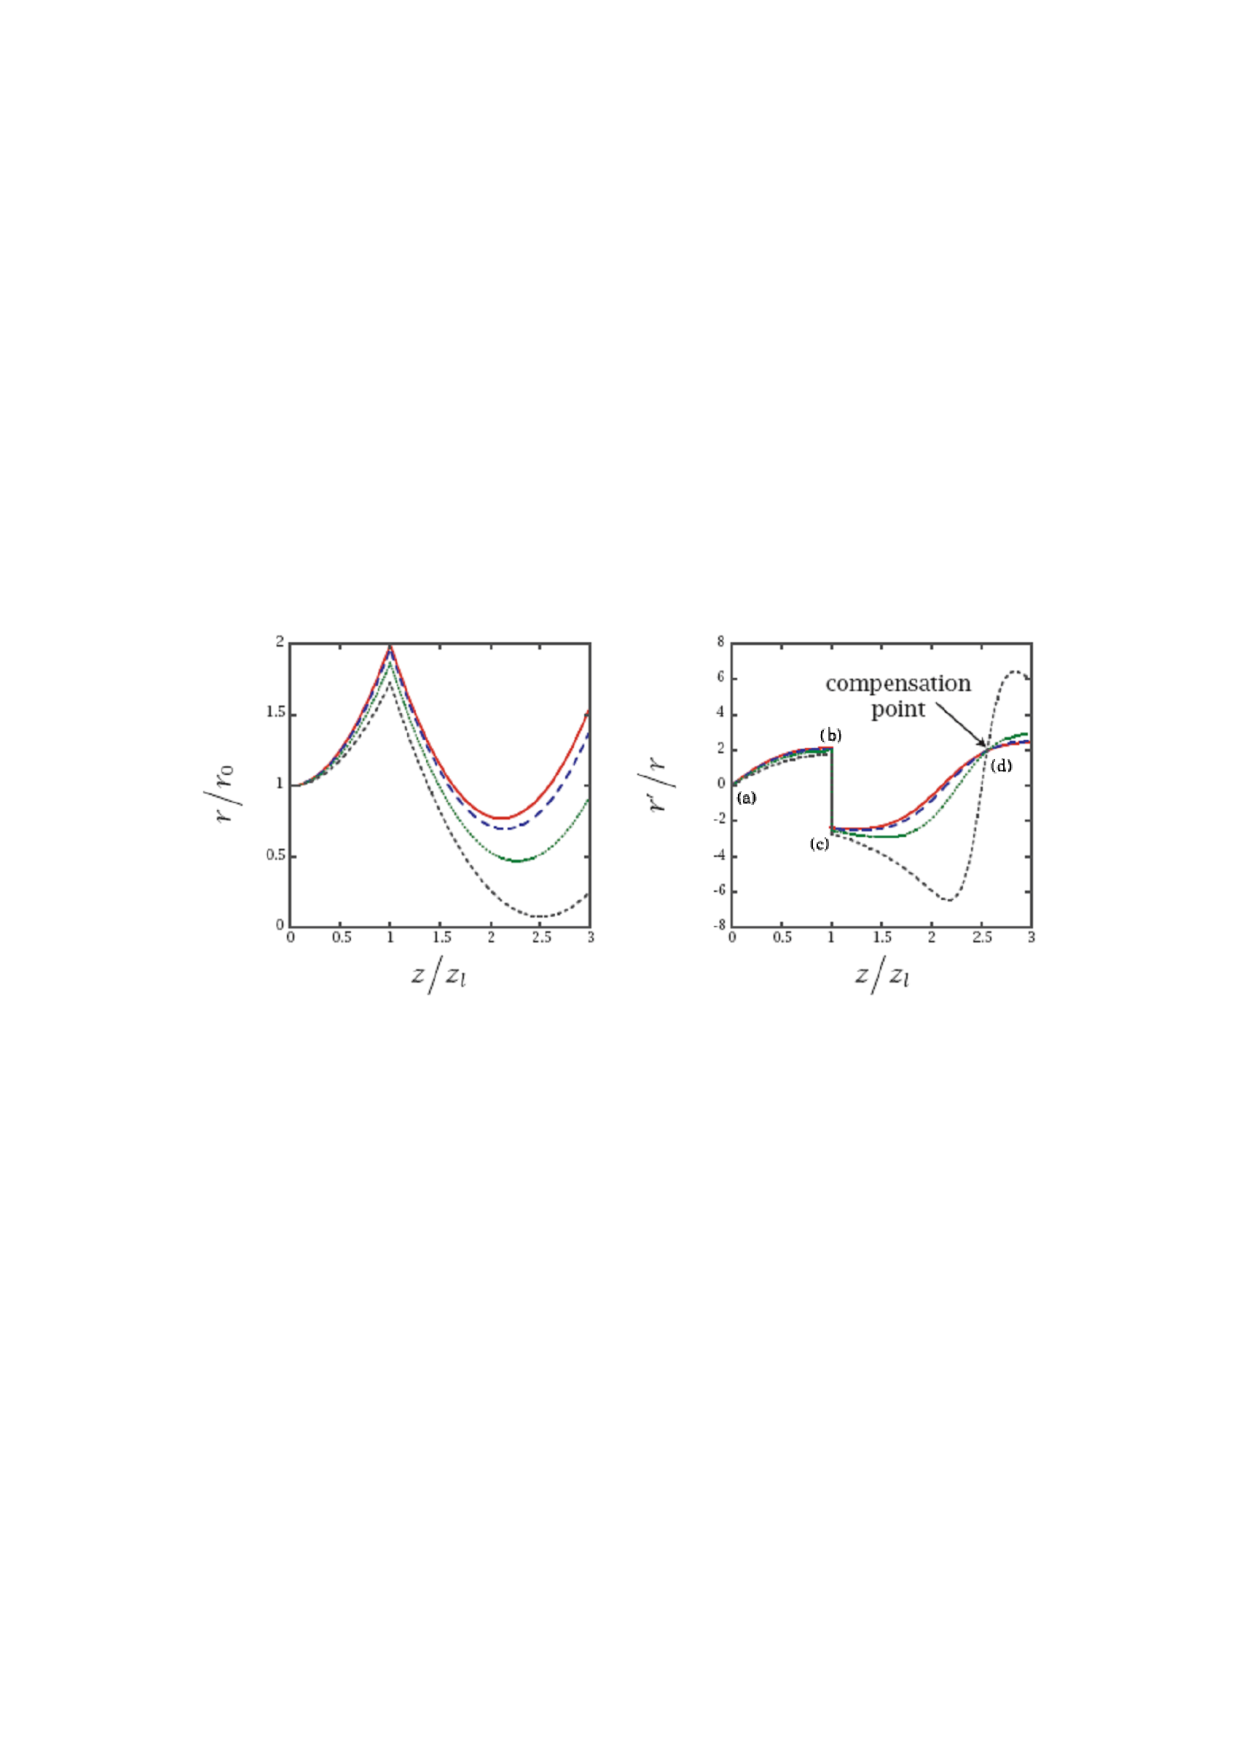
\includegraphics[width=0.9\textwidth]{solcomp}
\caption{\label{fig:solcomp} 螺线管线圈补偿线性发射度增长的原理示意图\cite{Anderson:2002ab}。}
\end{figure}

\subsection{非线性发射度增长的抑制}
对于非线性 RF 作用而言,抑制发射度增长一般采用对称化的电子枪设计以减少结构引入的非线性力;同时可以缩短束流长度,使束流所占微波相位上,微波场强度基本呈线性,以减小纵向高阶分量引入的横向非线性力;人们还提出一种空间叠合型双频电子枪的概念,通过将基模与高阶模重叠在同一个腔体内,达到将 RF 部分相位区间中场强线性化的目标。

对于非线性空间电荷力,目前常采用的方法是设法使束流为 KV 分布(Kapchinskij-Vladimirskij Distribution)\cite{Kapchinskij:1959aa},以从根本上消除非线性空间电荷力。常用的产生 KV 分布束流的方式有:三维激光整形,扁平束发射(pancake regime)和笔形束发射(cigar regime)。

\subsubsection{KV 分布、扁平束与笔形束}
三维 KV 分布即六维椭球面上的均匀分布,实空间体现为三维椭球均匀分布。下面用二维 KV 分布(横向四维椭球面上的均匀分布)为例,给出 KV 分布的形式及其基本性质。二维 KV 分布的形式如下:
\begin{equation}
f(x, y, x^{\prime}, y^{\prime}) = \frac{\lambda}{Q\pi^2\varepsilon_x\varepsilon_y}\delta\left[\left(\frac{x}{\sigma_x}\right)^2+\left(\frac{\sigma_x x^{\prime}-\sigma_x^{\prime} x}{\varepsilon_x}\right)^2+\left(\frac{y}{\sigma_y}\right)^2+\left(\frac{\sigma_x x^{\prime}-\sigma_x^{\prime} x}{\varepsilon_x}\right)^2\right]
\end{equation}
其中 $\lambda$ 为此纵向切片处的线电荷密度,$Q$ 为束团总电荷量。对 $(x^{\prime}, y^{\prime})$ 空间积分,就有:
\begin{equation}
n(x, y) = \frac{\lambda}{Q\pi\sigma_x\sigma_y},\quad (x/\sigma_x)^2+(y/\sigma_y)^2 < 1
\end{equation}
也即实空间中电荷均匀分布在一个椭球(椭圆)内部。KV 分布是唯一使各方向空间电荷力为线性的分布\cite{Kapchinskij:1959aa}。

扁平束即纵横比远小于 1 的束流,在发射过程中,由于其极强的纵向空间电荷力,扁平束流会在很短时间内纵向膨胀成为一个准 KV 分布束团;笔形束与扁平束正相反,它的纵横比远大于 1,是靠其极强的横向空间电荷力,在发射后迅速横向膨胀成为一个准 KV 分布束团。虽然扁平束和笔形束的最终形态都接近 KV 分布,但由于其膨胀过程是个强非线性过程,低的发射度在膨胀时可能会被破坏,所以产生 KV 分布最理想的办法就是用 KV 分布的激光入射直接产生 KV 分布的初始电子束,然而目前的激光技术尚不足以产生精度足够的三维椭球均匀分布的激光脉冲,因此消除非线性空间电荷力的技术依然处于发展中。

\subsubsection{抑制非线性力发射度增长中面临的问题}
非线性 RF 场发射度抑制与非线性空间电荷力发射度抑制之间存在矛盾:为抑制非线性空间电荷力发射度增长,需要将束团尽量拉长;然而拉长后的束团又在射频场中占有相当相位,这就会造成非线性 RF 场发射度的增长;反之亦然,缩短束团长度可以抑制非线性 RF 场发射度的增长,但也会造成初始非线性空间电荷力的增长。两者之间此消彼长。

克服二者的矛盾,可以:1)设法将射频场某相位区间的场强线性化,这也就是双频电子枪的基本想法;2)直接产生较长的 KV 分布的束团;3)提高阴极表面场强,抑制非线性空间电荷力发射度。然而以上三种办法均有自己的缺点:空间叠加型双频电子枪结构复杂,调谐困难;激光的三维整形技术尚不成熟,且由于阴极表面的镜像电荷效应,初始服从 KV 分布的束团若电荷量太大会出现畸变,因此只限于产生低流强的束团;阴极表面场强由电子枪对暗电流/打火等因素的容忍程度限制,不能无限制提高。如何更有效地抑制电子枪(或注入器)中的非线性力发射度增长,依然是一个研究热点。
